\documentclass[twocolumn,aps]{revtex4}

% allows special characters (including æøå)
\usepackage[utf8]{inputenc}
%\usepackage [norsk]{babel} %if you write norwegian
\usepackage[english]{babel}  %if you write english

\usepackage{physics,amssymb}  % mathematical symbols (physics imports amsmath)
\usepackage{graphicx}         % include graphics such as plots
\usepackage[table]{xcolor}
\usepackage{xcolor}           % set colors
\usepackage{hyperref}         % automagic cross-referencing 
\usepackage{float}			  % force placement of tables and figures
\usepackage{comment}
%\usepackage[authoryear]{natbib}
\usepackage{algorithm}
\usepackage{amsthm}
\usepackage{algpseudocode}
\usepackage{multirow}



\newtheorem{prop}{Proposition}[section]

\begin{document}

\title{A Study of Regularization and Resampling for High-Degree Polynomial Regression on a Sparse Data Set}
\date{\today}               
\author{
    Anton Nicolay Torgersen 
}
\affiliation{University of Oslo}


\newpage


%Abstract: accurate and informative? Total number of possible points: 5

    \begin{abstract}
This study conducts an empirical investigation into the performance of Ordinary Least Squares (OLS), Ridge, and LASSO regression for fitting high-degree polynomial models to Runge's function on a sparse dataset. 
We analyze the implementation of these regression models alongside various optimization algorithms and resampling techniques to understand their effectiveness in mitigating overfitting. 
Our findings indicate that no single model is universally superior; instead, performance is highly dependent on a thorough hyperparameter search and the choice of evaluation methodology. 
The study concludes that the key to achieving robust generalization on sparse data lies not in the selection of a specific model, but in the rigorous process of tuning and validation required to effectively manage the bias-variance tradeoff.
\end{abstract}


    \maketitle
    \thispagestyle{empty} % Removes page number from the title page

    


% Introduction: status of problem and the major objectives. Total number of possible points: 10
\section{Introduction}

The fundamental problem in machine learning and statistics is to find meaningful patterns in data using models that make accurate predictions on unseen data.
This is a difficult task, as a complex function might fit the training data perfectly, but fail spectacularly when facing new instances, a phenomenon known as overfitting.
On the other hand a model that is too simple may fail to extract the patterns in the data and thus underfit the data.
Therefore, understanding the bias-variance tradeoff on simpler models before working on more complex ones is paramount to develop robust and generalizable models.

This paper will study the bias-variance tradeoff through the lens of regression models, that increase in complexity.
We start with the simplest model, Ordinary Least Squares (OLS), where we have a fully analytical solution for the best fit parameters.
Then we move on to Ridge regression, which is a regularized version of OLS, where we first introduce the tuning of a penalization parameter $\lambda$ to find a good balance between bias and variance.
Finally we end with LASSO regression, which is another regularized version of OLS, but with a different penalization term.

This analysis will closely follow the lecture notes from FYS-STK3155 \cite{compfys} and the book "The Elements of Statistical Learning" by Hastie, Tibshirani and Friedman \cite{hastie}.
We will review the theory of the three regression methods and apply the methods to a one-dimensional problem, fitting a polynomial model to Runge's function, $f(x)=1/(1+25x^2)$.
This function is notoriously difficult for high-degree polynomial interpolation and will therefore be a good demonstration of the pitfalls of overfitting and the benefits of regularized techniques like Ridge and LASSO.
Together these three models will create a better understanding of the dynamics between bias and variance, how the dynamic shifts with model complexity and methods.
The result is a better intuition for tuning models, when is the model inching towards the true function $y$ and when is it stuck in a well. 

To conduct this investigation, our analysis is structured in two main parts. 
First, we will apply the regression models directly to the sparse dataset, beginning with the analytical solutions for OLS and Ridge before moving to iterative optimization methods like Gradient Descent for all three models. 
Second, we will employ resampling techniques—specifically bootstrap and cross-validation—to empirically quantify the bias-variance tradeoff and their performance on our dataset.


\section{Methods}\label{section:methods}
This section details the regression, optimization, and resampling techniques employed to analyze 
Runge's function, $$f(x)=1/(1+25x^2),$$ which is notoriously difficult for high-degree polynomial interpolation. 
We begin by describing data preparation, followed by the three regression methods and the gradient descent algorithms used for optimization.

\subsection{Data Preparation}
The fundamental data for this study was generated from Runge's function, $f(x)=1/(1+25x^2)$, with $x$ values uniformly distributed in the interval $[-1,1]$. 
The primary study utilized a sparse dataset of $N=18$ points to acutely demonstrate the high variance associated with overfitting. 

Two versions of the dataset were created: a noiseless set, used for the main analysis, and a noisy set generated by adding Gaussian stochastic noise, $\epsilon \sim N(0,0.1)$. 
The datasets were consistently split into training and test sets at an 80/20 ratio to evaluate generalization performance.

To ensure numerical stability and prevent coefficients corresponding to higher-degree polynomial terms from dominating the cost function, all features were scaled and centered by subtracting the mean value. 
This preprocessing step is critical, especially when dealing with regularization techniques, as it prevents the scale differences between polynomial features (e.g., $x$ vs. $x^{15}$) from skewing the optimization process.


\subsection{Regression Methods}
These methods aim to find a polynomial function $\tilde{y}(x)$ that approximates the true function $y(x)$, given a dataset of points $(x_i,y_i)$. 
This approximation is formulated linearly in terms of the parameters $\theta$ and the design matrix $X$: $\tilde{y}=X\theta$, where $X$ contains polynomial features of $x$. 
The analytical solutions for OLS and Ridge regression were implemented using custom code based on linear algebra operations.

\subsubsection{Ordinary Least Squares (OLS)}
OLS is the simplest method, aiming to find the parameter vector $\theta$ that minimizes the Mean Squared Error (MSE) cost function, $C(\theta)$, which represents the sum of the squared differences between observed values $y_i$ and predicted values $\tilde{y}_i$.
$$C(\theta)=\frac{1}{n}\sum_{i=1}^{n}(y_i-\tilde{y}_i)^2$$

Since the cost function is convex, minimizing the gradient provides a closed-form analytical solution, known as the normal equation. 
In implementation, the pseudoinverse function (numpy.linalg.pinv) was used to solve for the parameter vector $\theta$:
$$\theta=(X^TX)^{-1}X^Ty$$

This solution is valid provided that $X^TX$ is invertible. The gradient used for iterative optimization is:
$$\nabla_{\theta_n}=\frac{1}{n}2X^T(X\theta_n-y)$$



\subsubsection{Ridge Regression}
Ridge regression introduces L2 regularization, adding a penalty term proportional to the square of the magnitude of the parameters $\theta_j$ to the OLS cost function.
$$
C(\theta, \lambda) = \frac{1}{n} \sum_{i=1}^{n} (y_i - \tilde{y}_i)^2 + \lambda \sum_{j=1}^{p} \theta_j^2
$$

Here, $\lambda \geq 0$ is the regularization hyperparameter controlling the strength of the penalty. 
The analytical solution now becomes:
$$
\theta=(X^TX+\lambda I)^{-1}X^Ty,
$$

where $I$ is the identity matrix.

The gradient for iterative optimization is:
$$
\nabla_{\theta_n}=\frac{1}{n}2X^T(X\theta_n-y)+2\lambda\theta_n
$$


\subsubsection{LASSO Regression}
LASSO (Least Absolute Shrinkage and Selection Operator) regression employs L1 regularization, penalizing the sum of the absolute values of the parameters, which encourages sparsity.
$$
C(\theta, \lambda)=\frac{1}{n}\sum_{i=1}^{n}(y_i-\tilde{y}_i)^2+\lambda\sum_{j=1}^{p}|\theta_j|
$$

Because the L1 penalty term is not differentiable at $\theta_j=0$, an analytical solution does not exist. 
This necessitates the use of iterative optimization techniques such as proximal gradient descent.
This is done by first calculating the gradient for the OLS part of the cost function, and then applying a soft-thresholding operator to the parameters after each gradient step:
$$\theta_{n+1} = S_{\lambda}(\theta_n - \eta \nabla_{\theta_n})$$
where $\eta > 0$ is the learning rate and $S_{\lambda}$ is the soft-thresholding operator defined as:
$$S_{\lambda}(\theta_j) = \text{sign}(\theta_j) \max(|\theta_j| - \lambda, 0)$$

For more on these three methods see chapter 2 in \cite{compfys} and Section 3.4.1-2 in \cite{hastie}.
\subsection{Gradient Descent}
Iterative optimization methods are employed, primarily Gradient Descent (GD), where the parameter vector $\theta$ is updated iteratively based on the negative gradient of the cost function and a learning rate $\eta$: $\theta_{n+1}=\theta_n-\eta\nabla_{\theta}$.


\subsubsection{Changing learning rate algorithms}
Four advanced optimization algorithms were implemented to iteratively update the learning rate, primarily focusing on OLS and Ridge models due to similarities in their gradient formulation.
These methods modify the standard gradient descent step, $\theta_{t+1}=\theta_t-\eta\nabla_{\theta} J(\theta_t)$, by adapting the learning rate ($\eta$) or the direction ($\nabla_{\theta} J(\theta_t)$).
\\ 

\textbf{Momentum}

Accelerates gradient descent by incorporating a fraction of the previous update ($v_t$) into the current step, smoothing the optimization path and helping to maintain consistent descent:
\begin{align*}
v_{t+1} &= \beta v_t + (1 - \beta) \nabla_{\theta} J(\theta_t) \\
\theta_{t+1} &= \theta_t - \eta v_{t+1}
\end{align*}
Where $v_t$ is the velocity term and $\beta$ is the momentum hyperparameter.
\\

\textbf{Adagrad}

Adapts the learning rate for each parameter by scaling it inversely proportional to the cumulative sum of all past squared gradients ($G_t$). This approach effectively shrinks the learning rate for frequently updated parameters:
\begin{align*}
\theta_{t+1} &= \theta_t - \frac{\eta}{\sqrt{G_t + \epsilon}} \odot \nabla_{\theta} J(\theta_t)
\end{align*}
where $G_t$ is the diagonal matrix containing the sum of squared gradients up to time $t$, and $\epsilon$ is a small constant for numerical stability.
\\

\textbf{RMSprop}

Addresses the aggressive, monotonic decay of ADAgrad by using an exponentially decaying moving average of the squared gradients, $E_t$, which helps prevent the learning rate from diminishing too quickly in later iterations:
\begin{align*}
\theta_{t+1} &= \theta_t - \frac{\eta}{\sqrt{E_t + \epsilon}} \odot \nabla_{\theta} J(\theta_t)
\end{align*}
where $E_t$ is the moving average of the squared gradients.
\\

\textbf{Adam}

Combines the strengths of Momentum and RMSprop, maintaining both a moving average of the gradients ($m_t$, the first moment) and a moving average of the squared gradients ($v_t$, the second moment). 
ADAM is often considered the most stable and efficient general-purpose optimizer. 
The update rules are:

\begin{align*}
m_{t+1} &= \beta_1 m_t + (1 - \beta_1) \nabla_{\theta} J(\theta_t) \\
v_{t+1} &= \beta_2 v_t + (1 - \beta_2) (\nabla_{\theta} J(\theta_t))^2 \\
\theta_{t+1} &= \theta_t - \frac{\eta}{\sqrt{v_{t+1}}} \odot m_{t+1}
\end{align*}
where $\beta_1$ and $\beta_2$ are decay rates for the moments.
\\

The implementation of these methods on the OLS and Ridge methods followed a straightforward approach, with the gradients calculated as described earlier.
See section E and the GitHub repository \cite{rep} for the exact implementation.

For more on the theory around these methods see chapter 7 in \cite{compfys}.
\subsubsection{Stochastic Gradient Descent}
Stochastic Gradient Descent (SGD) is an optimization method that approximates the full batch gradient by utilizing a small, randomly sampled subset of the data, known as a mini-batch $B_t$ of size $m$, at each iteration. This introduces stochastic noise into the optimization path. 
The parameter update relies on the mini-batch gradient $\nabla_{\theta_t}$, calculated here for OLS:
$$\nabla_{\theta_{t}}=\frac{2}{m}\mathbf{X}_{B_{t}}^{T}(\mathbf{X}_{B_{t}}\theta_{t}-\mathbf{y}_{B_{t}})$$
The parameters $\theta$ are then updated iteratively using a fixed learning rate $\eta$:
$$\theta_{t+1}=\theta_{t}-\eta\nabla_{\theta_{t}}$$

For regularized methods like Ridge and LASSO, the respective regularization terms are incorporated into the gradient calculation or applied using a proximal step (for LASSO) before the update. This study employed a mini-batch size of $m=6$ on the sparse dataset ($N=18$).

\subsection{Sampling methods}
The empirical quantification of model error is essential for evaluating generalization performance and understanding the factors contributing to total predictive error. The decomposition of the expected Mean Squared Error (MSE), proven in \ref{prop:BiasVarianceDecomp}, confirms that the total error is composed of squared bias, variance, and irreducible noise ($\sigma^2$).

\begin{prop}
For a model $\tilde{y}$ that approximates the true function $y=f(x)+\epsilon$, the expected mean squared error can be decomposed into three components: the variance of the model, the squared bias of the model, and the variance of the noise.
$$\mathbb{E}[(y-\tilde{y})^2]=\mathrm{Bias}[\tilde{y}]^2+\mathrm{Var}[\tilde{y}]+\sigma^2$$
\label{prop:BiasVarianceDecomp}
\end{prop}

\begin{proof}

Expand $\mathbb{E}[(y-\tilde{y})^2]$ as follows:
\begin{align*}
\mathbb{E}[(y-\tilde{y})^2 ]&= \mathbb{E}[(y-\tilde{y}) (y-\tilde{y}) ] \\
&= \mathbb{E}[(y^2-\tilde{y} y -y \tilde{y} +\tilde{y}^2)] \\
&= \mathbb{E}[y^2] - 2 \mathbb{E}[\tilde{y} y] +\mathbb{E}[\tilde{y}^2] \\
\end{align*}

Looking into the function $\mathbb{E}[\tilde{y}^2]$ and using $\mathrm{var}[\tilde{y}] = \mathbb{E}[\tilde{y}^2] - \mathbb{E}[\tilde{y}]^2$ we see that this can be written as
$$
\mathbb{E}[\tilde{y}^2] = \mathrm{var}[\tilde{y}] + \mathbb{E}[\tilde{y}]^2.
$$

Secondly, replacing $y$ as $f + \varepsilon$ in $\mathbb{E}[y^2]$, where we are assuming $f$ to be non stochastic and $\varepsilon \sim N(0, \sigma^2)$, we get:
$$
\mathbb{E}[(f+\varepsilon)^2] = \mathbb{E}[f^2] + 2 \mathbb{E}[f]\mathbb{E}[\varepsilon] + \mathbb{E}[\varepsilon^2] =  f^2 + \sigma^2
$$

Lastly the term $\mathbb{E}[\tilde{y} y]$, becomes the following as $\tilde{y}$ and $\varepsilon$ are assumed independent.
$$
\mathbb{E}[\tilde{y} (f + \varepsilon)] = \mathbb{E}[\tilde{y} f] + \mathbb{E}[\tilde{y} \varepsilon] = f \mathbb{E}[\tilde{y}] + 0
$$

Putting everything together we get:
\begin{align*}
&=\mathbb{E}[y^2] - 2 \mathbb{E}[\tilde{y} y] +\mathbb{E}[\tilde{y}^2] \\
&= f^2 + \sigma^2 - 2 f \mathbb{E}[\tilde{y}] +\mathrm{var}[\tilde{y}] + \mathbb{E}[\tilde{y}]^2 \\
&= f^2 - 2 f \mathbb{E}[\tilde{y}] + \mathbb{E}[\tilde{y}]^2 + \mathrm{var}[\tilde{y}] + \sigma^2 \\
&= \mathbb{E}[ (f - \mathbb{E}[\tilde{y}])^2] + \mathrm{var}[\tilde{y}] + \sigma^2 \\
&= \mathrm{Bias}[\tilde{y}]^2  + \mathrm{Var}[\tilde{y}] + \sigma^2 \
\end{align*}

Where we have approximated $f$ with the noisy $y$, in the last step in order to practically estimate the bias.
\end{proof}

The following resampling techniques provide the necessary frameworks to estimate these components empirically.

\subsubsection{Bootstrap}
The Bootstrap method, which means random sampling with replacement, is employed here primarily to generate the multiple model realizations required to empirically calculate the bias and variance components, as depicted in Figure \ref{fig:biasvariance}. 
Although Bootstrap yields a theoretically low bias estimate because it trains models using samples of size N, the use of sampling with replacement can lead to higher variance in the error estimate, particularly when applied to small or sparse datasets, where the duplication of influential points heavily skews the resulting model parameters.

\subsubsection{Cross Validation}
$k$-fold Cross-Validation (CV) is a widely preferred technique for estimating generalization error due to its robust nature, producing predictions for all data points exactly once.
In $k$-fold CV, the dataset is partitioned into $k$ mutually exclusive subsets, or folds. 
The model is iteratively trained on $k-1$ folds and tested on the remaining fold, repeating the process $k$ times. 
The final generalized MSE is calculated as the average of the test errors obtained from each rotation.

The systematic nature of CV, which involves sampling without replacement, ensures that the test folds are entirely independent from the training sets. 
This methodology typically results in a lower variance estimate of the test error compared to Bootstrap. 
While training occurs on a slightly smaller effective dataset ($N(k-1)/k$), which might introduce a minimal increase in bias compared to training on the full dataset, this increase is often offset by the significant stability gained in the variance estimation. 

These two techniques are applied across all three regression methods—OLS, Ridge, and LASSO—to provide a stable, comparable metric of generalization performance.
For more information on bootstrap and cross-validation see section 7.10-11 in \citet{hastie} or chapter 3 in \citet{compfys}.


\subsection{Implementation and Code}
The code for this project was written in Python, utilizing libraries such as NumPy for numerical computations, Matplotlib for plotting, and Scikit-learn for some machine learning functionalities.

There are two main files, utils.py and ResultGeneration.ipynb.
The utils.py file contains functions for generating data, creating polynomial features, and implementing the analytical regression methods (OLS and Ridge) as well as the calculation of the gradient.
Though much of the code for the different optimization algorithms are written directly in the ResultGeneration.ipynb file, under the section it belongs to.

The ResultGeneration.ipynb file is a Jupyter notebook that is structured into different sections generating the results and plots for each part of this research paper.
It is structured to allow modification of parameters such as the number of data points, polynomial degree, regularization strength, learning rate, and number of iterations. All results and plots are generated directly from this notebook with a fixed random seed ensuring reproducibility.



\subsubsection{Testing and Comparison}
To ensure correctness in the implementation of the metrics and the analytical solutions for OLS and Ridge regression, the results were cross-validated against Scikit-learn's built-in functions.
Here we saw that the results matched quite well for both the metrics MSE and R2 score, as well as the actual parameter values $\theta$ in the ridge and OLS methods.
For the MSE and R2 score the results were identical, while the parameters $\theta$ matched up to a precision of $10^{-14}$.
See the GitHub repository \cite{rep} Code/ResultGeneration.ipynb for the comparison results.

When it comes to the gradient implementations, they were not directly compared to Scikit-learn, but the convergence behavior and final MSE values were monitored to ensure they aligned with theoretical expectations and the results from the analytical methods.

\subsection{Use of AI tools}
While working on generating the results for this project the auto-completion tool github copilot has been used in order to speed up the coding process.
It has been used to generate code snippets and functions based on the context of the code being written.
Gemini has also been used in order to debug and find errors in the code.

After having generated the results, we have used Gemini to help in assessing and improving the quality of the report.
Reducing grammatical errors and improving the clarity and flow of the text.
In the github repository for this project one can see the commit history and when the different AI tools have been used.
\begin{figure*}[t]
    \centering  
    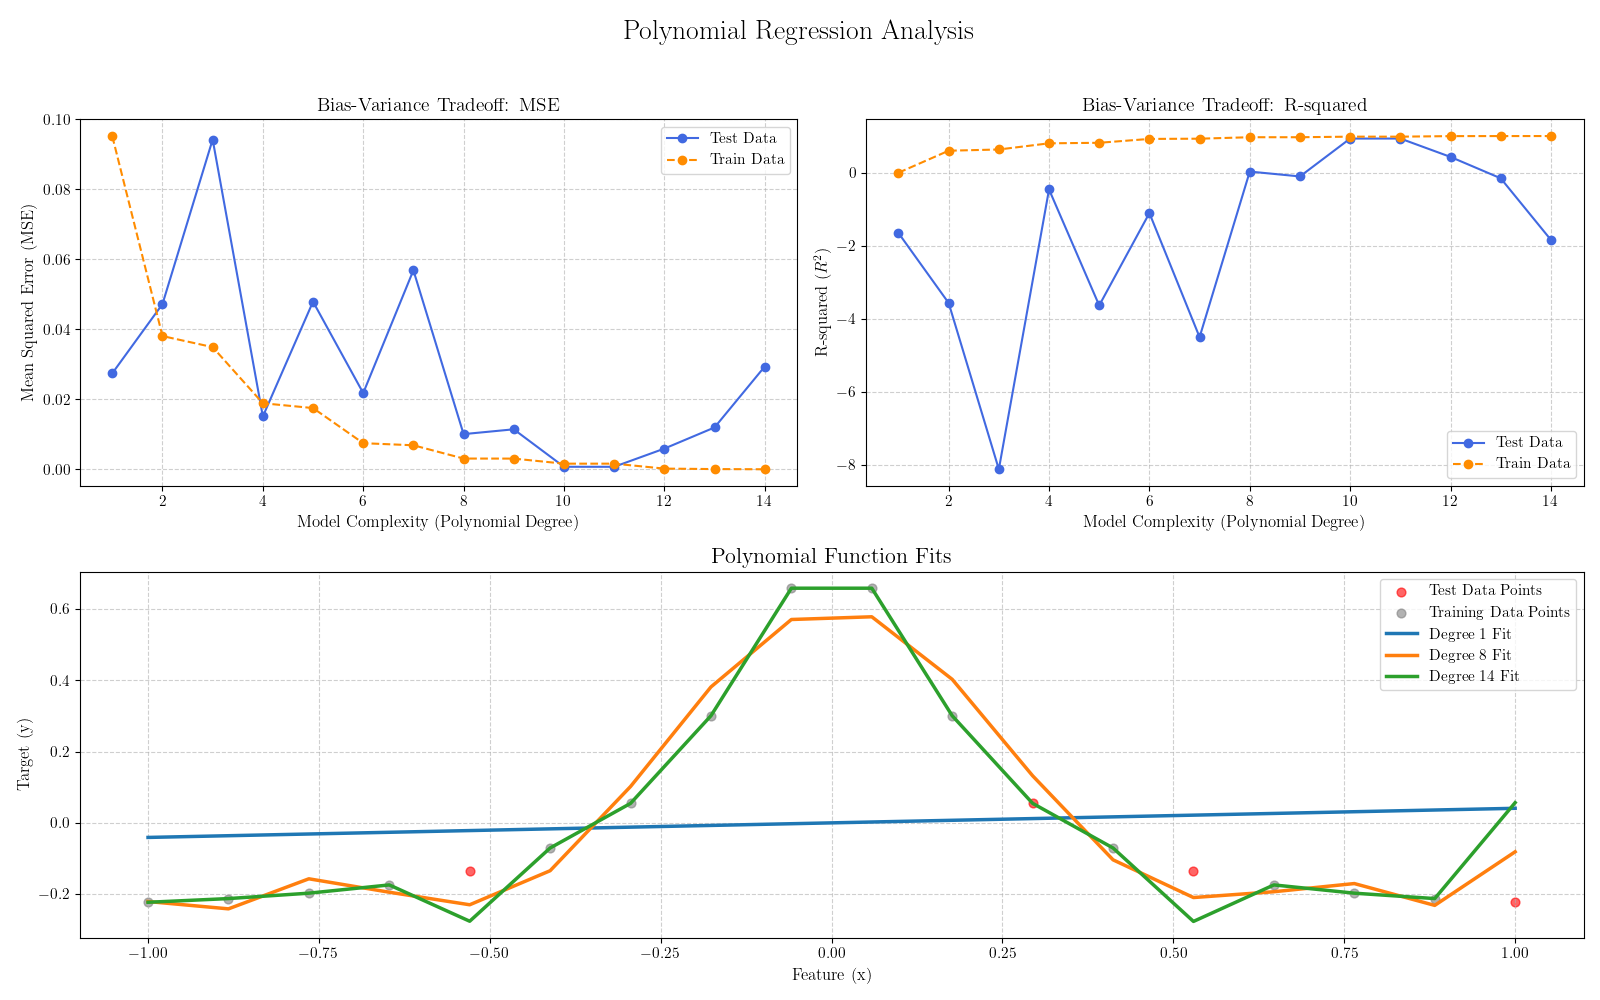
\includegraphics[width=.95 \linewidth]{Figures/Combined_Analysis_OLS.png}
    \caption{OLS and model complexity ($N=18$)}
    \label{fig:OLS1}
\end{figure*}
\section{Results and Discussion}\label{section:results}
The results we are going to focus on and visualize are related to the true values instead of those with added noise. 
Since what we found in our analysis are that the results are mostly the same except for worse performance when using the noisy data.
One exception where the analytical solutions for OLS and Ridge, where one clearly saw that the noise had a lot of effect on the solutions as OLS was very prone to overfitting and Ridge was a bit more robust.
But since our analysis will be around a sparse dataset we will be using the noiseless one for the main analysis.

\subsection{Analytical Regression methods}

\subsubsection{Ordinary Least Squares (OLS)}

We first applied OLS regression to the sparse dataset (N=18) generated from Runge’s function. 
This initial analysis, illustrated in \ref{fig:OLS1}, reveals the failure of OLS to generalize as model complexity (polynomial degree p) increases. 
As we see that the higher lines perfectly hits the training points and ignores the underlying function, by jumping up and down near the test points.

One sees that the Training MSE approaches zero as complexity increases because the model has enough parameters to interpolate every training data point. 
However, the Test MSE increases past a polynomial degree of 12, as we see that the model fits the points rather than the function.
The R2 score on the test set confirms this, by going from an acceptable value to something that is increasing downwards, confirming that the model fails to generalize.

An observation with regards to noise, i.e. more noise makes the model more prone to miss the function as the points no longer matches perfectly. This is especially pronounced in our case as there are so few points and the model will become even more confused on what the underlying pattern is.
\begin{figure}[H]
    \centering
    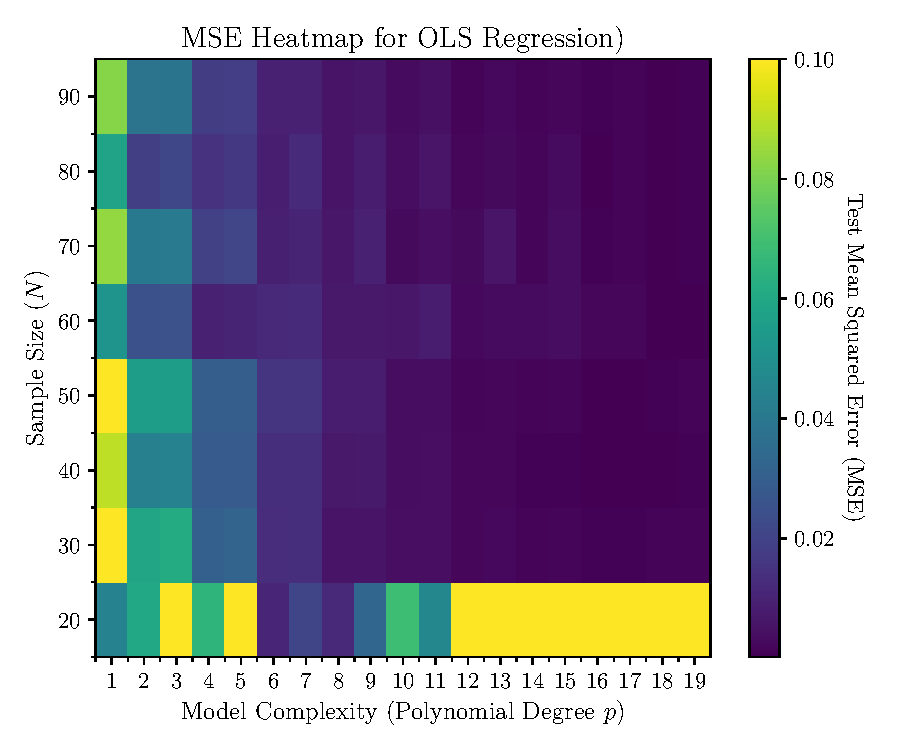
\includegraphics[width=.95 \linewidth]{Figures/OLS_Heatmap.pdf}
    \caption{OLS data size and model complexity}
    \label{fig:OLSHeat}
\end{figure}


The heatmap \ref{fig:OLSHeat} shows that the highest Mean Squared Error (MSE), occurs in the region characterized by high complexity (p) and low sample size (N). 
This region, exhibiting yellow spots, demonstrates where the bias-variance trade-off tilts entirely towards variance and numerical instability. 
Conversely, increasing the sample size (moving up the x-axis) significantly stabilizes the MSE for higher polynomial degrees. 
This confirms that adding more data intrinsically reduces the model's sensitivity to random fluctuations (variance) because the model has better information to distinguish between signal and noise, thereby allowing for the successful use of more complex models.

Looking closer at figure\ref{fig:OLSHeat} we see, as we expect, along the borders where there is low training data or low complexity are the worst performing parts on the test data. 
These yellow spots are especially pronounced as these are points where the training is prone to diverge just as the graph \ref{fig:OLS1} is beginning to do at $p=14$.
Especially in the left corner we see a clear case of when the tradeoff between bias and variance goes towards low bias and high variance.


\subsubsection{Ridge Regression}
Doing the same training but using Ridge as our method we got some interesting results that elucidates the differences between these models.
Both has their improvements increasing as the complexity increases, but the differences are in the lows and the highs.
Where the OLS method\ref{fig:OLS1} had a really low value at degree 10, it also begins to diverge more abruptly at degree 14.
The Ridge method on the other hand doesn't have the same lows as OLS, but it also doesn't diverge as abruptly as OLS.
Implying that the regularization terms is doing its job and keeps the model from fitting the training data to closely.


\begin{figure}[h]
    \centering
    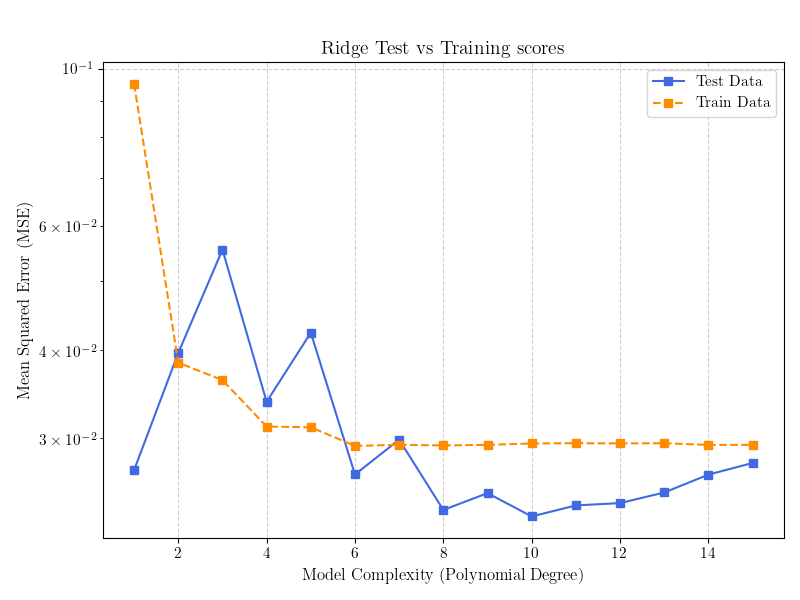
\includegraphics[width=.95 \linewidth]{Figures/MSE_RidgeOnly.png}
    \caption{Ridge and model complexity ($\lambda=0.001$)}
    \label{fig:RidgeMse}
\end{figure}


\begin{figure}[h]
    \centering
    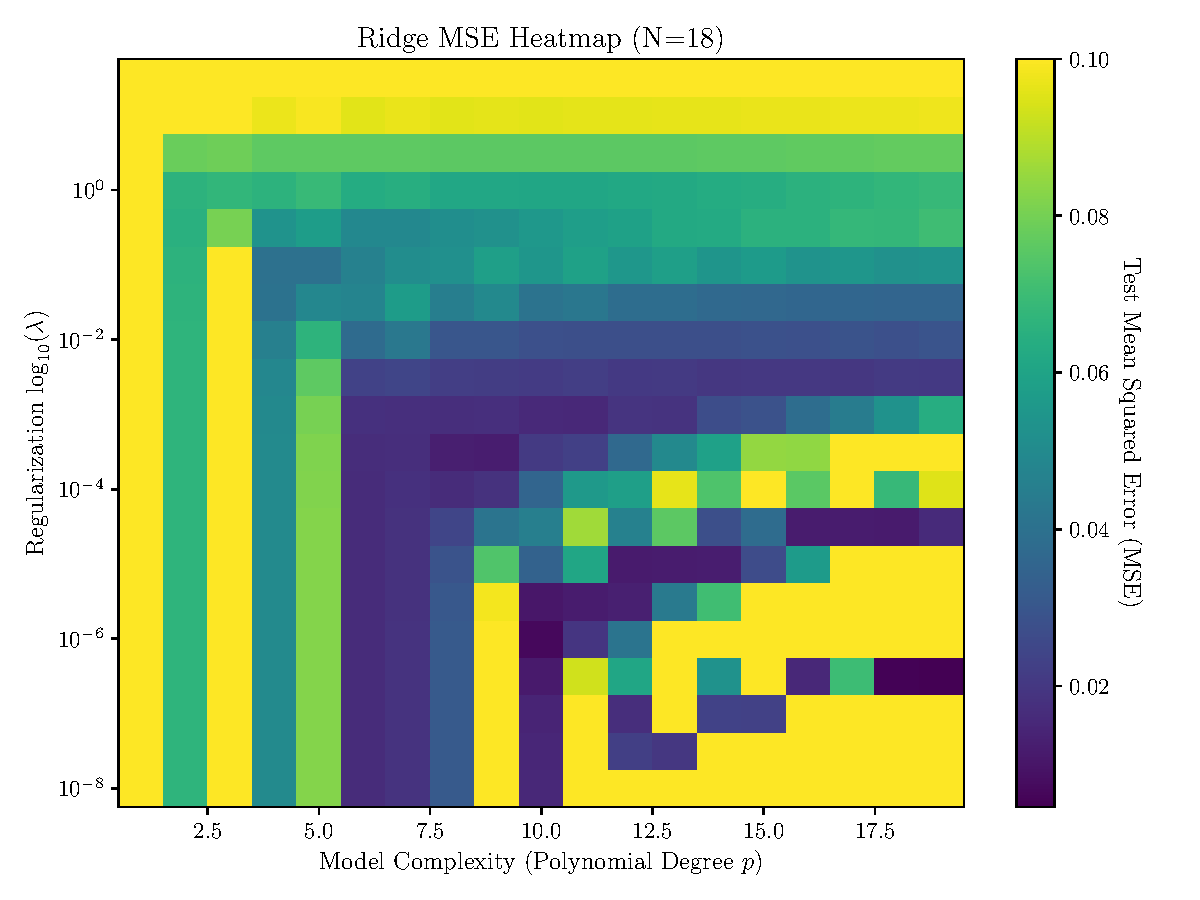
\includegraphics[width=.95 \linewidth]{Figures/Ridge_Degree_Lambda_Heatmap.pdf}
    \caption{Ridge Regularization and model complexity}
    \label{fig:RidgeHeat}
\end{figure}


To better understand how regularization strength ($\lambda$) interacts with model complexity, we can examine the heatmap in Figure \ref{fig:RidgeHeat}. 
This plot visualizes the test MSE across a range of polynomial degrees and $\lambda$ values. 
Where we see that when the model is too simple (low p) or the regularization is too strong (high $\lambda$), the model underfits, resulting in high bias and poor performance.

The most insightful feature of the heatmap is the distinct arching pattern, which traces the "valley" of the optimal $\lambda$ for each polynomial degree.
For any given polynomial degree, a $\lambda$ that is too small (below the valley) fails to control the model's high variance, leading to overfitting.
Conversely, a $\lambda$ that is too large (above the valley) introduces excessive bias, causing the model to underfit by failing to capture the underlying patterns in the data.

Ultimately, the position of these arches demonstrates a core principle of machine learning: that finetuning hyperparameters like $\lambda$ is crucial for balancing bias and variance, especially as model complexity increases.


\subsection{Using Gradient Descent}

\subsubsection{OLS and Ridge with gradient descent}
The first application of Gradient Descent with a fixed learning rate of $\eta=0.01$ for both Ordinary Least Squares (OLS) and Ridge regression confirmed that optimization required a substantial number of iterations before reaching a minimum\ref{fig:DescOLSRidge}.

Where Ridge in comparison to OLS would reach a plateau or begin to stabilize near the end, OLS will still contain some development at this point. 
Some for the better and some for the worse.

We also observed that the models had different iterations where MSE was minimized.
One notable instance is OLS-12 which had an early minimum right before 1,000 iterations, then decreased in performance, though it looks like it might find a better minimum after some more iterations.
We also see that for most of the time the complex models are just as good as the linear ones implying that the models are struggling to learn the function.


\begin{figure}[h]
    \centering
    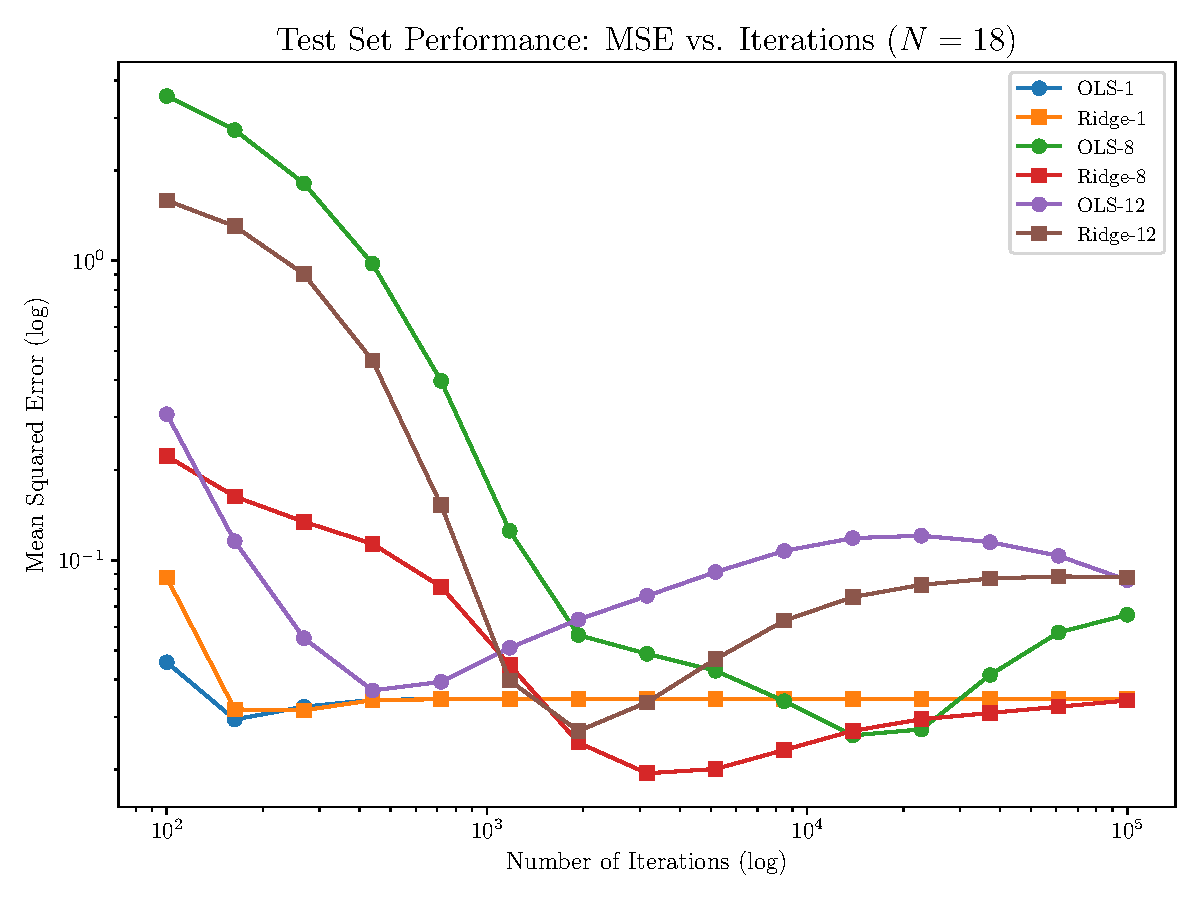
\includegraphics[width=.95 \linewidth]{Figures/Gradient_Comparison_OLS_Ridge_18.pdf}
    \caption{Gradient descent for OLS and Ridge ($\eta=.01, \lambda=.001$)}
    \label{fig:DescOLSRidge}
\end{figure}
Our analysis on the learning rate $\eta$ revealed that both excessively low and high values were detrimental to convergence.
A learning rate much lower than 0.01 resulted in prohibitively slow convergence, while rates at 0.1 and higher led to instability in the training.

Therefore $\eta=0.01$ was ultimately selected as the hyperparameter for the remainder of the project's analysis. 
This rate was chosen as a robust compromise between optimization speed and stability.
Meaning that the rest of the graphs in this paper will be using this learning rate for better visual comparisons.


\subsubsection{LASSO Regression}
Utilizing Lasso regression with the same parameters and dataset we get some interesting results see figure \ref{fig:Lasso1}.
In comparison to ridge and OLS, Lasso show a much more stable downwards trajectory on the same learning rate.
Where it will, similarly to Ridge, also begin to plateau at some point, but in our case it was much later than Ridge.

When we did the same training with a learning rate of $0.1$ we saw that the model will begin to plateau more quickly but with a miniscule improvement on the performance on the test set. 
Here we saw that Lasso-12 in figure \ref{fig:Lasso1} will plateau slightly above Lasso-8, with a small minimum before the plateau.


\begin{figure}[h]
    \centering
    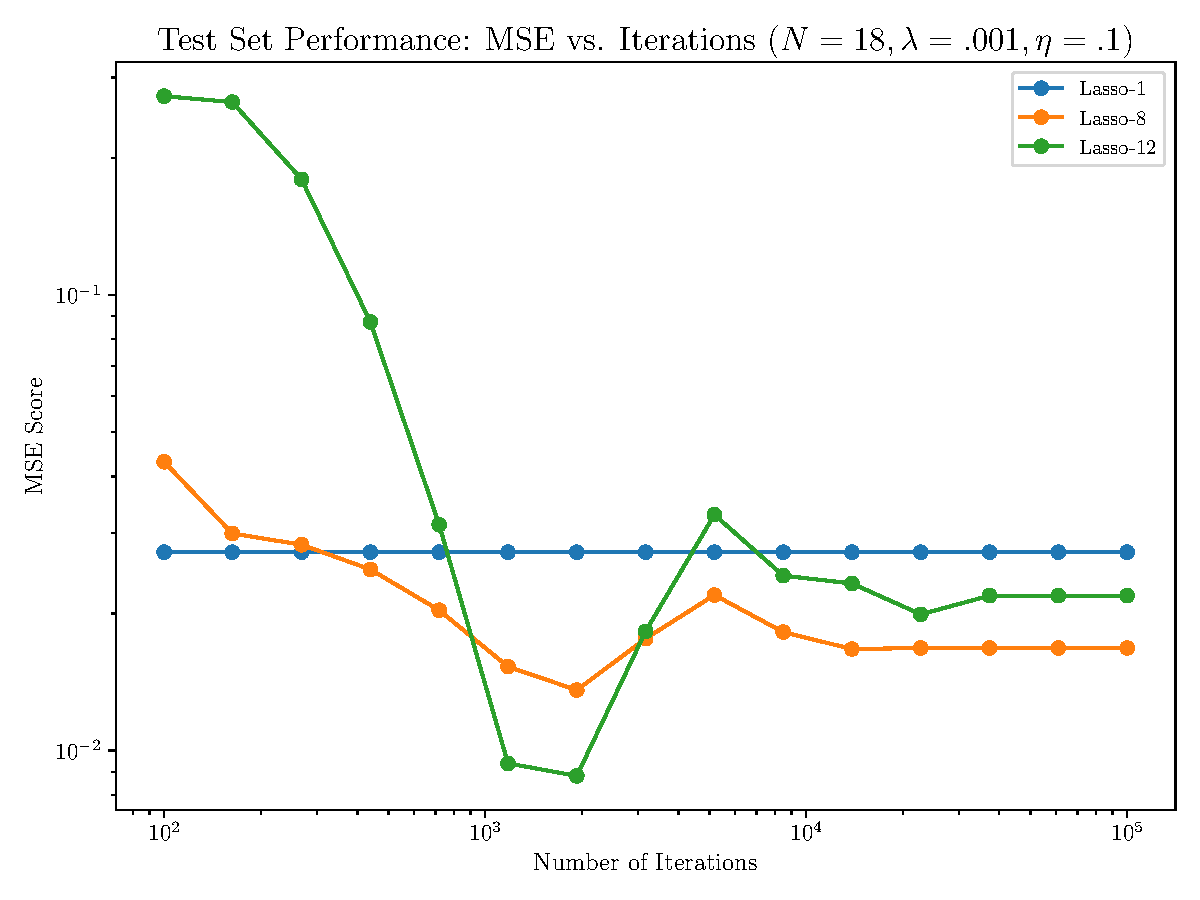
\includegraphics[width=.95 \linewidth]{Figures/Lasso_MSE.pdf}
    \caption{Lasso learning ($\eta=.01, \lambda=.001$)}
    \label{fig:Lasso1}
\end{figure}

A comparative analysis of the convergence plots offers insight into the nature of the models themselves. The instability of the high-degree OLS model (OLS-12) in Figure \ref{fig:GradSGD}, which finds an early minimum before diverging, is a direct consequence of its high-variance nature creating an ill-conditioned and chaotic loss landscape. 
The optimizer struggles to navigate this terrain, overshooting the minimum.

In stark contrast, LASSO's stable convergence in Figure \ref{fig:Lasso1} can be attributed to the simplifying effect of the L1 penalty. By driving many coefficients to exactly zero, LASSO performs implicit feature selection. 
This simplifies the effective model being optimized, resulting in a smoother, better-behaved loss landscape that allows the optimizer to descend to a minimum more reliably.

\subsection{Comparative Analysis of Adaptive Learning Rates}

For simplicity in implementation, we exclusively used OLS and Ridge methods here, given their similar gradient descent implementations. 
We utilized the same dataset of $N=18$ points and a fixed learning rate of $\eta=0.01$ for baseline gradient descent. 
The hyperparameters for the different methods were kept consistent across all figures to facilitate comparison.

\subsubsection{Momentum}

Our initial approach to adaptive learning rates involved implementing a momentum term in the gradient descent algorithm. 
In early trials, a high momentum term led to high volatility in the training process. 
Reducing the momentum to $0.6$ yielded the results shown in Figure 7. 
We observe that the momentum term generally aids models in reaching their minimum faster.
A quick comparison between figure \ref{fig:DescOLSRidge} and figure \ref{fig:GradMomentum} shows that theses two figures are quite similar just that the momentum one is shifted slightly left.
It also improved on the performance at the end results of the plateau for the ridge models.
While for the OLS-12 model we now see that the downward trajectory has continued and reached a new minimum after $10^5$ iterations.
\\
\begin{figure}[h]
    \centering
    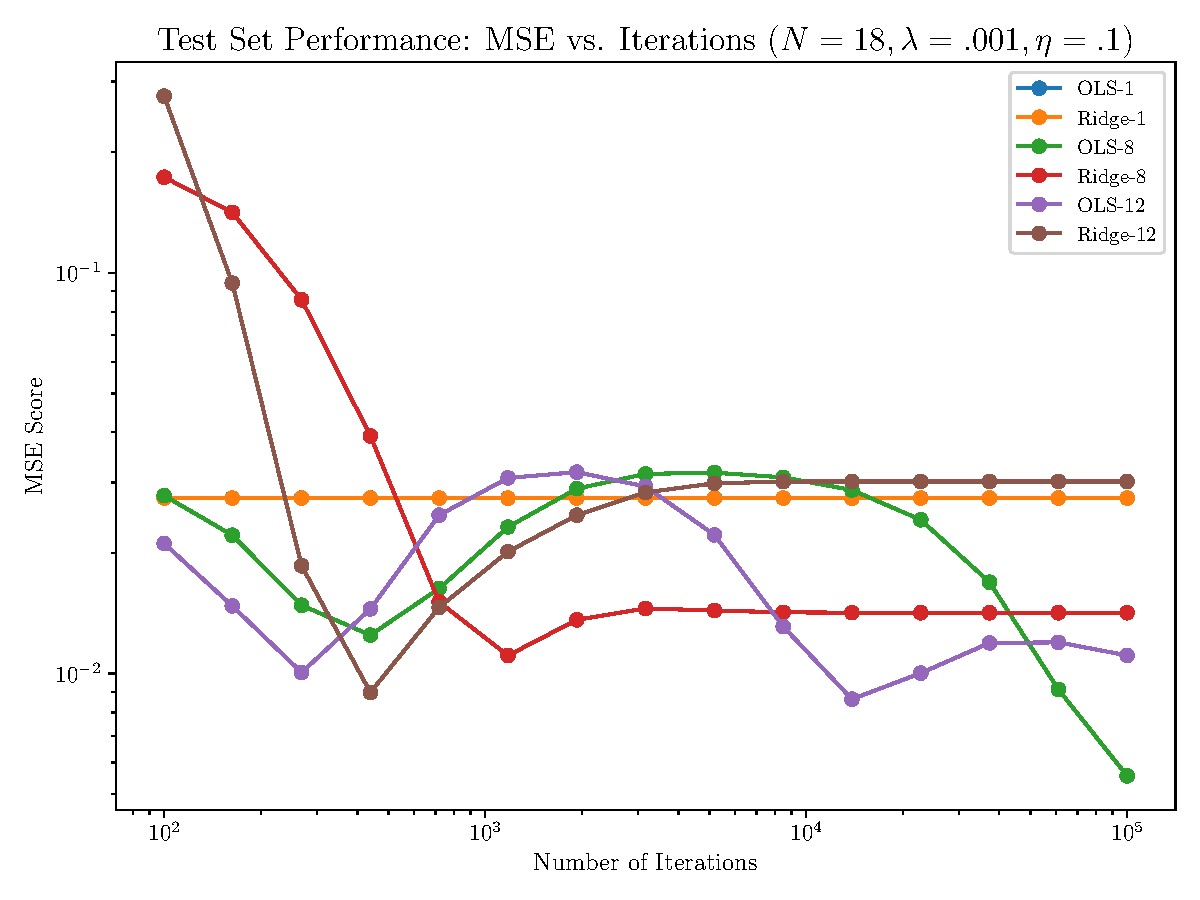
\includegraphics[width=.95 \linewidth]{Figures/OLS_Ridge_Momentum.pdf}
    \caption{Gradient descent with momentum ($\eta=.01, \lambda=.001, \beta=0.6$)}
    \label{fig:GradMomentum}
\end{figure}


\subsubsection{ADAgrad}

The results from the ADAgrad method are displayed in Figure \ref{fig:GradADAgrad}. 
Compared to the momentum method or basic gradient descent, ADAgrad exhibits notably slower convergence, though it is almost always in a positive direction towards a better minimum. 
This behavior is primarily attributed to ADAgrad's mechanism, where the learning rate starts relatively small and progressively diminishes with cumulative squared gradients.
At the end of our training runs we see that the models are nearing a bottom, which is near what we got in momentum and normal gradient descent.
Remarkably enough even the linear models take a long time to converge here.
\\

\begin{figure}[h]
    \centering
    \includegraphics[width=.95 \linewidth]{Figures/OLS_Ridge_ADAgrad.pdf}
    \caption{Gradient descent with ADAgrad ($\eta=.01, \lambda=.001$)}
    \label{fig:GradADAgrad}
\end{figure}


\subsubsection{RMSprop}
When we look at our results for RMSprop, they are much more volatile as seen in figure \ref{fig:GradRMSprop}.
Though there is a clear difference between OLS and Ridge here, where OLS swings a lot while Ridge seems to act more stable though revolving up and down in a cyclic manner.
An other interesting observation is that we know see a much better performance on the OLS-8 model, where we have the lowest MSE of all the models and the previous gradient methods.
\\

\begin{figure}[h]
    \centering
    \includegraphics[width=.95 \linewidth]{Figures/OLS_Ridge_RMSprop.pdf}
    \caption{Gradient descent with RMSprop ($\eta=.01, \lambda=.001, \beta=0.9$)}
    \label{fig:GradRMSprop}
\end{figure}

\subsubsection{Adam}

The Adam optimization method, which combines the strengths of both momentum and RMSprop, exhibits a noticeable reduction in volatility compared to the other three adaptive methods, as illustrated in Figure \ref{fig:GradADAM}. 
The oscillations in MSE scores are less pronounced, which could indicate a more stable optimization trajectory.
Though in our case most of the models seems stuck at a plateau except for OLS-12 that now has reached a new lowest point after $10^5$ iterations, and if we where to run it longer it might have climbed down even further.
What is interesting is that compared to RMSprop, Adam has OLS-12 as it's best performing model just as in the momentum method.
\\

\begin{figure}[h]
    \centering
    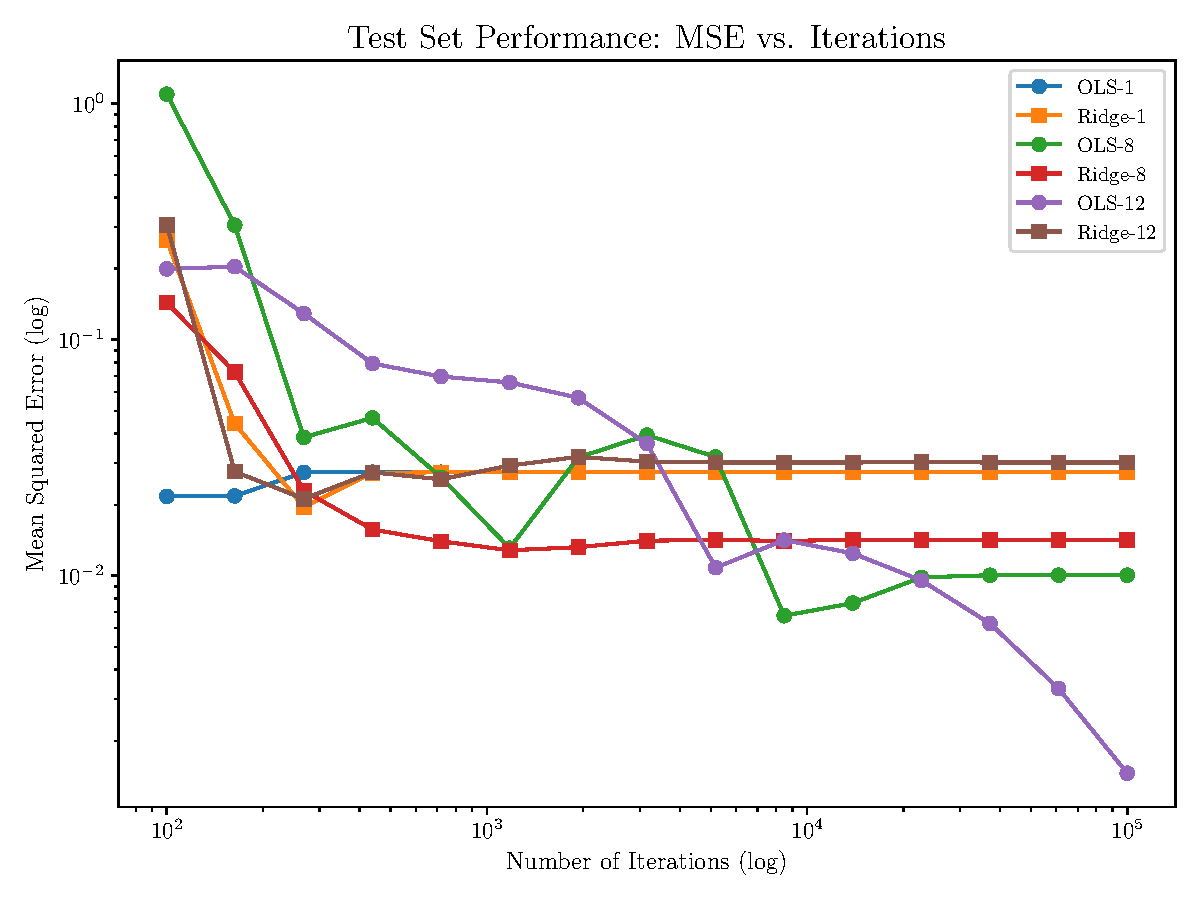
\includegraphics[width=.95 \linewidth]{Figures/OLS_Ridge_ADAM.pdf}
    \caption{Gradient descent with ADAM ($\eta=.01, \lambda=.001, \beta=0.9,\beta_2=0.999$)}
    \label{fig:GradADAM}
\end{figure}


\subsection{Stochastic Gradient Descent}

The results from the Stochastic Gradient Descent (SGD) method show a surprisingly effective performance on the sparse dataset. While one might intuitively expect increased volatility, the stochasticity appears to facilitate the discovery of lower error minima for certain models.

Specifically, the more complex polynomial models, such as Ridge-12 and OLS-12, achieve remarkably low minimum Mean Squared Error scores. This performance for higher-degree polynomials is notably better than that of simpler models. This suggests that the noise inherent in SGD's updates helps these complex models navigate the loss landscape and escape shallow local minima, leading to improved generalization.

In contrast, the OLS-8 model settles at a noticeably higher error compared to the lower minima found by the most complex models. 
The overall outcome highlights that for this sparse dataset, SGD, particularly for more complex models like Ridge-12 and OLS-12, can effectively find better solutions, as it finds a lower performance better than the standard method.


\begin{figure}[h]
    \centering
    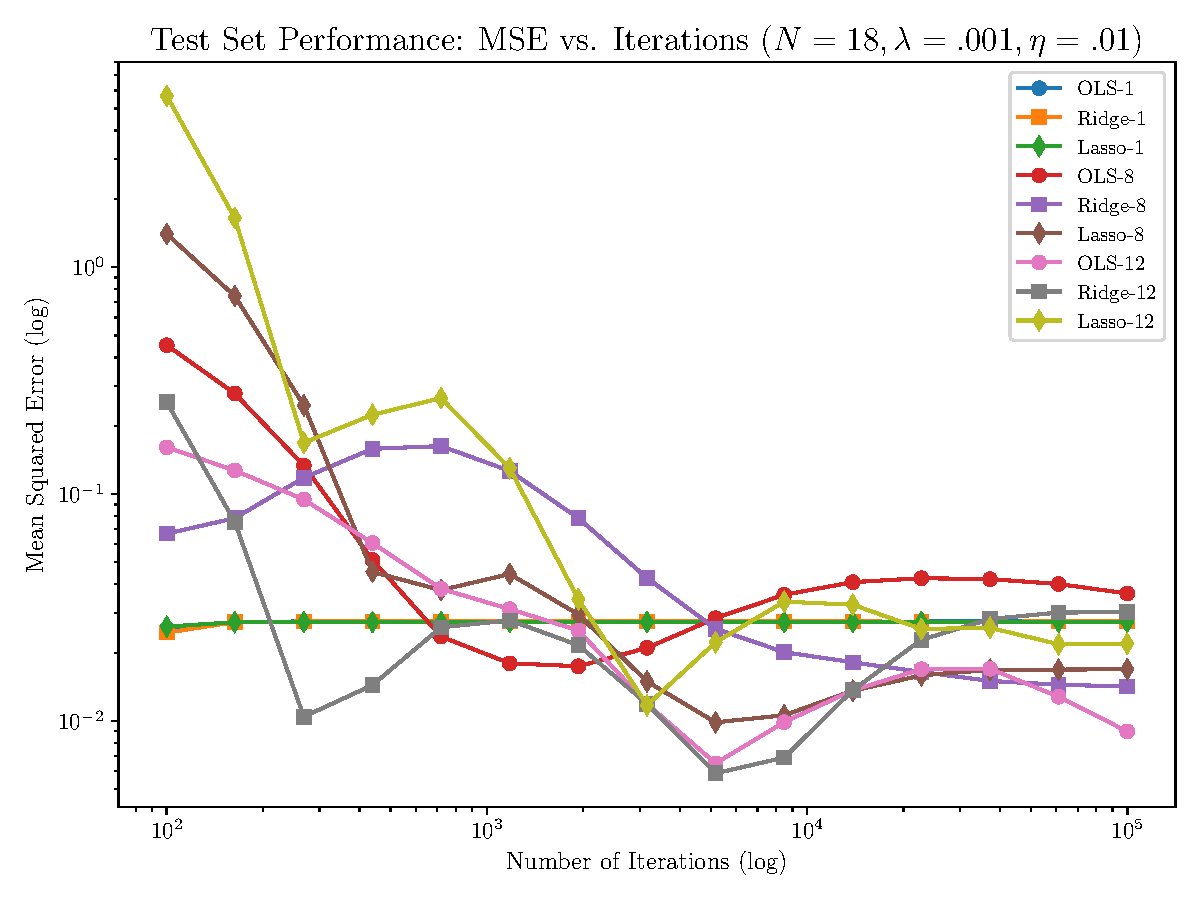
\includegraphics[width=.95 \linewidth]{Figures/StochasticDescent.pdf}
    \caption{Stochastic Gradient Descent ($\eta=.01, \lambda=.001, m=6$)}
    \label{fig:GradSGD}
\end{figure}
\subsection{Resampling Techniques}
The preceding analyses confirmed that fitting high-degree polynomials to the Runge function with Ordinary Least Squares (OLS) on a sparse dataset ($N=18$) leads to extreme high variance and overfitting. 
This phenomenon is visually captured in Figure \ref{fig:OLS1}, where complex models diverge significantly, and even the linear model exhibits learned bias, particularly failing to capture test data near $x=1$. 
To address this instability and better quantify the bias-variance trade-off, this section evaluates the use of resampling techniques to build a more robust and generalizable model.

\begin{figure}[h]
    \centering
    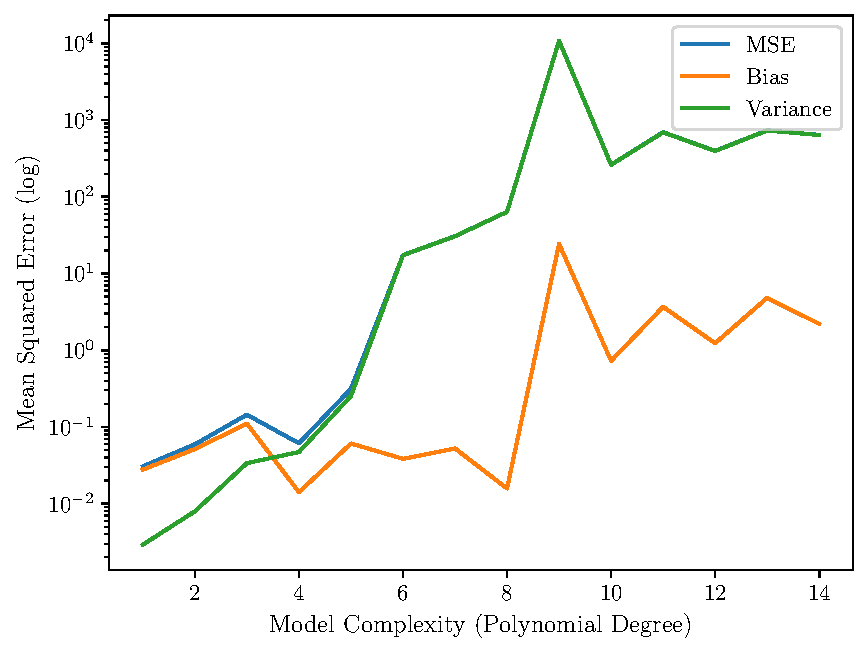
\includegraphics[width=.95 \linewidth]{Figures/bias_variance_tradeoff.pdf}
    \caption{Bias-Variance Tradeoff}
    \label{fig:biasvariance}
\end{figure}

\subsubsection{Bootstrap}

\begin{figure}[h]
    \centering
    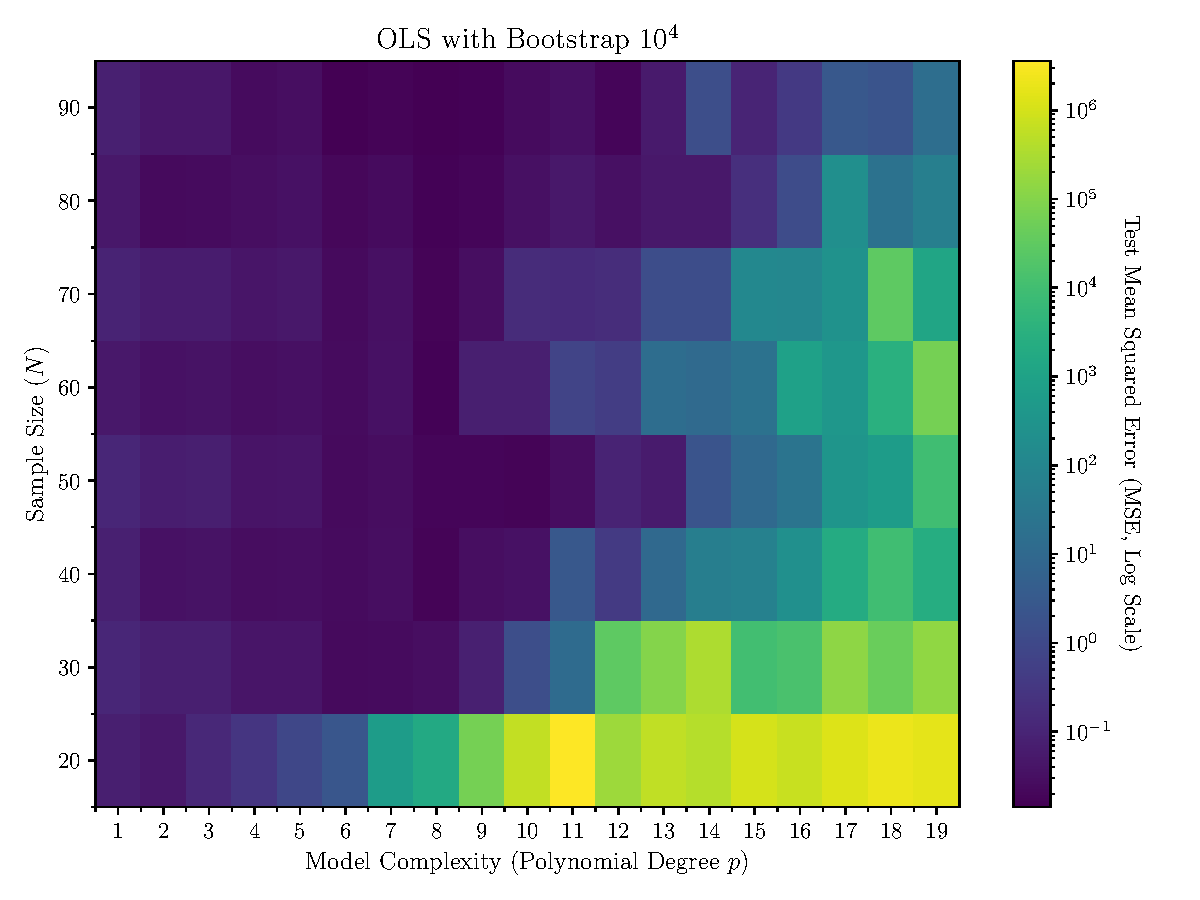
\includegraphics[width=.95 \linewidth]{Figures/Bootstrap_Heatmap.pdf}
    \caption{Bootstrap Heatmap}
    \label{fig:BootstrapHeatmap}
\end{figure}

Using bootstrap we do not see any improvements and instead it becomes remarkably worse on our small dataset.
This is likely due to the fact that the model is already overfitting the training data, and adding more noise through bootstrapping on a sparse dataset only exacerbates this issue.
Especially since bootstrapping uses sampling with replacement, meaning that some data points will be repeated multiple times in the training set.
Which means that the weight of the training will drastically change from one side of the function to the other, as the model is so sensitive to changes in the data.
We see this in figure \ref{fig:BootstrapPerformance} where the MSE is much higher than the previous methods.

Though when we use bootstrapping on all three models we find that Ridge and Lasso performs remarkably better than OLS in this method.
This is likely due to the fact that the regularization terms help to prevent overfitting, and therefore the model is less sensitive to changes in the data.
Lasso performs the best out of the three methods, likely due to the fact that it can set some coefficients to zero, effectively performing feature selection and reducing model complexity.


\begin{figure}[h]
    \centering
    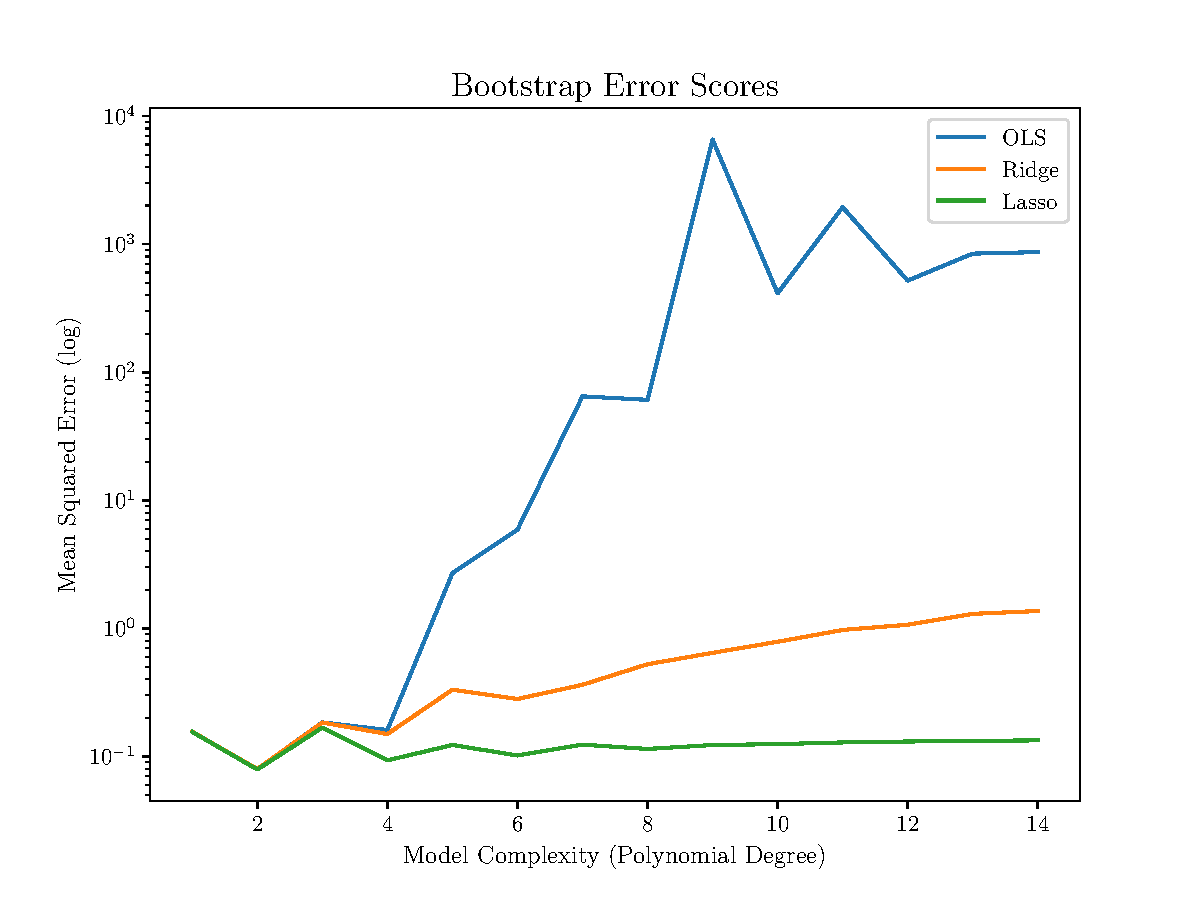
\includegraphics[width=.95 \linewidth]{Figures/Bootstrap.pdf}
    \caption{Bootstrap Performance ($\lambda=.001$)}
    \label{fig:BootstrapPerformance}
\end{figure}

If we where to look at the heatmap of the bootstrap results \ref{fig:BootstrapHeatmap} we see that the model is performing worst in the area where we are working in.
Implying that this is a poor method for this dataset with variables close to the amount of data points.


\subsubsection{Cross Validation}
5-fold Cross-Validation (CV) worked better on all the models as seen in figure \ref{fig:CrossValidation}, and gave a lower MSE than bootstrap did.
Especially for OLS it prevented the model from blowing up so quickly when the model complexity increased.

The systematic, non-replacement partitioning of data in CV yields a more reliable error estimate than Bootstrap.
This makes sense as the we will train on more unique data points, rather than resampling the same points multiple times.
Reducing the percentage of unique training points to a much higher degree because of the small dataset.

Ridge and Lasso are sticks closer together in CV especially remarkable is that the Lasso model seems to plateau when we increase the complexity.
A particularly insightful result is that Ridge regression achieved the lowest overall MSE with Cross-Validation, whereas LASSO was the top performer under the Bootstrap method. 
This suggests an interaction between the resampling technique and the properties of the regularizer. 
Bootstrap's sampling-with-replacement on a small dataset can create training sets with high collinearity between polynomial features (e.g., if a single data point is duplicated multiple times). 
Ridge (L2 regularization) is known to handle such multicollinearity effectively by shrinking the coefficients of correlated predictors together. 
In contrast, the more stable, non-replacement folds of CV produce less collinearity, creating a scenario where Ridge's smooth shrinkage provides a better-tuned solution than LASSO's more aggressive and potentially unstable feature selection.


\begin{figure}[h]
    \centering
    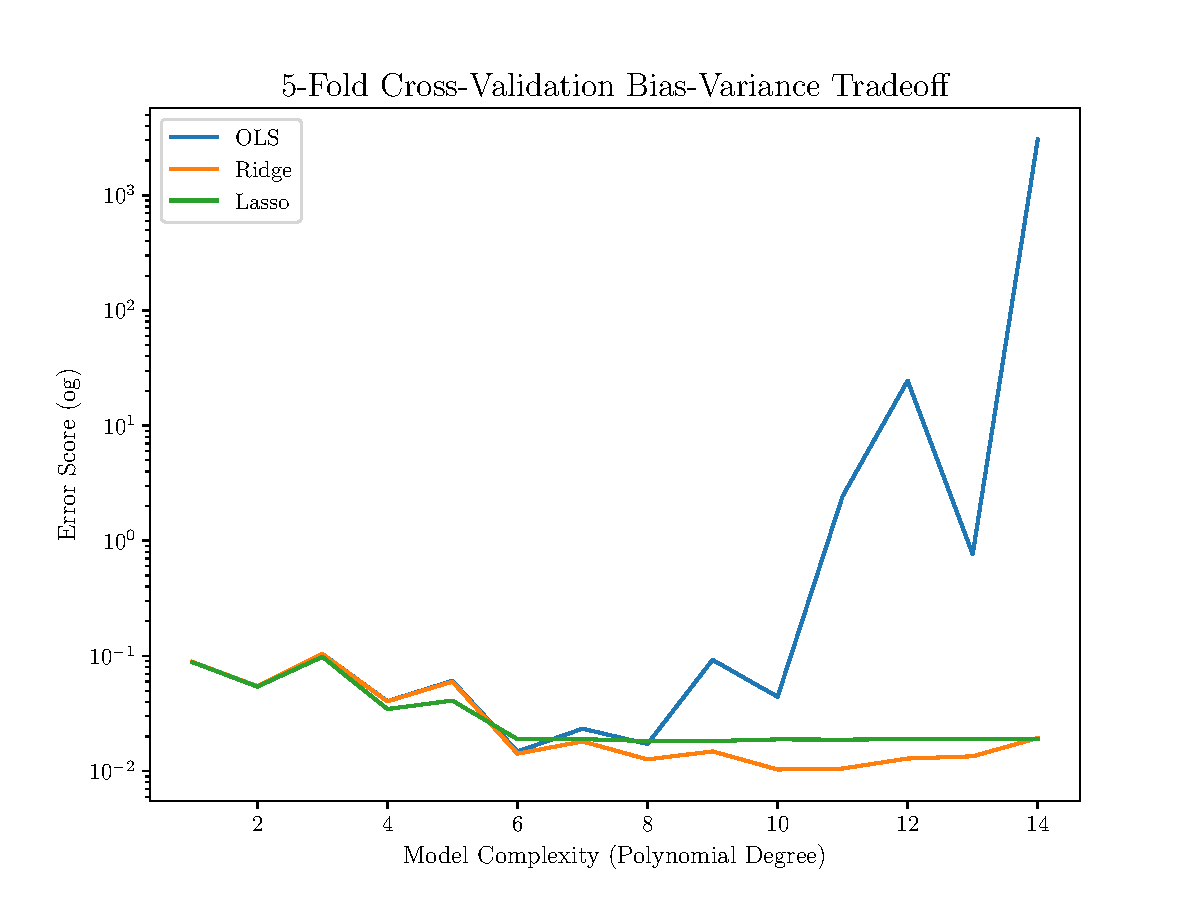
\includegraphics[width=.95 \linewidth]{Figures/Cross_Validation.pdf}
    \caption{5-fold Cross Validation ($\lambda=.001$)}
    \label{fig:CrossValidation}
\end{figure}

\section{further work}

\textbf{Hyperparameters analysis for optimizers}:
\\
While we compared several optimizers, their own hyperparameters (e.g., learning rate schedules, momentum terms) were held constant, in this discussion.
A more exhaustive grid search on these parameters could potentially unlock even better performance and reveal deeper insights into the optimization process for these specific regression problems and the size of the dataset.
Just as we saw with the regularization lines in figure \ref{fig:RidgeHeat}, we might find optimal hyperparameter regions for each optimizer and model complexity.
\\

\textbf{Impact of noise}
\\
This study focused on a noiseless dataset for clarity and since we wanted to understand the underlying relationships without the confounding effects of noise.
A valuable extension would be to quantify how different levels of stochastic noise influence the optimal regularization parameter ($\lambda$) and the relative performance of Ridge versus LASSO. 
\\

\section{Conclusion}\label{section:conclusion} 

This study demonstrates that for high-degree polynomial regression on sparse data, the choice of a specific model is secondary to the rigorous process of hyperparameter tuning and methodical validation. Our analysis of Runge's function reveals that the high variance inherent in complex, unconstrained models like Ordinary Least Squares (OLS) creates a chaotic and ill-conditioned loss landscape. This not only leads to severe overfitting (Figure \ref{fig:OLS1}) but also hinders the convergence of standard optimization algorithms.

The introduction of L1 (LASSO) and L2 (Ridge) regularization proved to be the critical first step in taming this complexity. By penalizing large coefficients, these methods effectively smooth the loss landscape, creating a more stable environment where optimizers can find meaningful minima. This stability was further enhanced by adaptive optimizers; the robust performance of Adam (Figure \ref{fig:GradADAM}) and the surprising effectiveness of Stochastic Gradient Descent (Figure \ref{fig:GradSGD}) highlight that the optimization strategy is as crucial as the model itself. SGD, in particular, leveraged its inherent noise to escape shallow local minima and achieve some of the best results for high-degree models.

Furthermore, our findings underscore the paramount importance of the validation method. On a sparse dataset, the sampling-with-replacement strategy of bootstrap proved detrimental, as the frequent duplication of influential data points exacerbated the model's tendency to overfit (Figure \ref{fig:BootstrapPerformance}). In contrast, the systematic, non-replacement partitioning of k-fold Cross-Validation provided a far more reliable estimate of generalization error, proving itself to be an indispensable tool for model selection and tuning in a low-data regime (Figure \ref{fig:CrossValidation}).

Ultimately, this work illustrates that achieving a generalizable model is not about finding a single 'best' algorithm, but about mastering the interplay between model complexity, regularization, optimization, and validation. A failure in any one of these areas can compromise the entire modeling process.

\bibliography{biblio}

% \appendix with table of hyperparameters and values for the models
\end{document}
